% \documentclass{article}

% % if you need to pass options to natbib, use, e.g.:
%     % \PassOptionsToPackage{numbers, compress}{natbib}
% % before loading neurips_2021

% \PassOptionsToPackage{numbers, sort}{natbib}
% %\usepackage[numbers,sort]{natbib}

% % ready for submission
% \usepackage{neurips_2021}

% % to compile a preprint version, e.g., for submission to arXiv, add add the
% % [preprint] option:
% %     \usepackage[preprint]{neurips_2021}

% % to compile a camera-ready version, add the [final] option, e.g.:
% %     \usepackage[final]{neurips_2021}

% % to avoid loading the natbib package, add option nonatbib:
% %    \usepackage[nonatbib]{neurips_2021}

% \usepackage[utf8]{inputenc} % allow utf-8 input
% \usepackage[T1]{fontenc}    % use 8-bit T1 fonts
% \usepackage[colorlinks]{hyperref}     % hyperlinks
% \usepackage{url}            % simple URL typesetting
% % \usepackage{booktabs}       % professional-quality tables
% \usepackage{amsfonts}       % blackboard math symbols
% \usepackage{nicefrac}       % compact symbols for 1/2, etc.
% \usepackage{microtype}      % microtypography
% \usepackage{xcolor}         % colors

% % added by me
% \usepackage{xcolor}
% % \usepackage{subfig}
% \usepackage{caption}
% \usepackage{amsmath}
% \usepackage{amssymb}
% \usepackage{multirow}
% \usepackage{graphicx}
% \usepackage{booktabs}
% \newcommand{\op}[1]{\operatorname{#1}}
% \newcommand{\mbf}[1]{\mathbf{#1}}
% \newcommand{\gowthami}[1]{\textcolor{red}{#1}}
% \newcommand{\bayan}[1]{\textcolor{cyan}{#1}}
% \newcommand{\micah}[1]{\textcolor{purple}{#1}}
% \newcommand{\tomg}[1]{\textcolor{blue}{#1}}


% \usepackage{algorithm}
% \usepackage{listings}
% \usepackage{wrapfig,booktabs}
% \usepackage{multirow}

% \usepackage{caption}
% \usepackage{subcaption}
% \usepackage{mathtools}


% \title{Appendix for SAINT: Improved Neural Networks for Tabular Data via Row Attention and Contrastive Pre-Training}
% \begin{document}

% \maketitle
\appendix
\textbf{\Large{Appendix for SAINT: Improved Neural Networks for Tabular Data via Row Attention and Contrastive Pre-Training}}

\section{Additional illustrations}
\label{appendix_sec:extra_illustrations}

\begin{figure}[h]
  \centering
  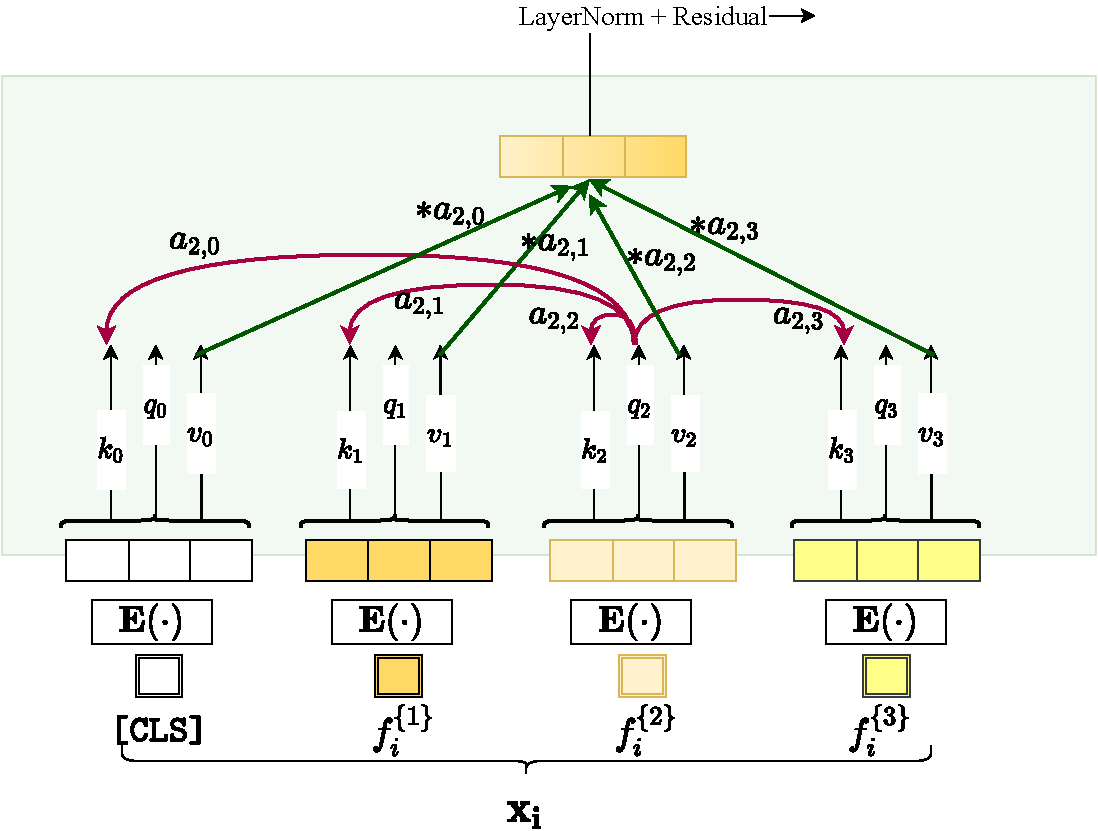
\includegraphics[width=\textwidth]{figs/appendix/selfattention.pdf}
  \caption{An illustration of self-attention in a point $\mathbf{x_i}$. Inspired by Vaswani et al~\cite{vaswani2017attention}.}
  \label{fig:self_attention_illustration}
\end{figure}

\section{Datasets}
\label{appendix_sec:datasets}


\textbf{Data sources} For each dataset, details and download links are listed in Tables \ref{tab:dataset_details} and \ref{tab:datasetlinks}. The 1995 Income Classification dataset is from a 2019 Kaggle competition and was made public without a license. The Arcene dataset, furnished by UCI \cite{Dua:2019}, comprises anonymized patient records, where the goal is to classify entries as containing cancer patterns or normal patterns \cite{guyon2004result}. The Arrhythmia dataset is made available by Stonybrook University \cite{liu2008isolation, ting2009mass, keller2012hics}. The Bank Marketing dataset is also compiled and organized by UCI and released for research use \cite{moro2014data}. The BlastChar dataset is fictitious, it is also part of a Kaggle competition and was originally generated by IBM \cite{ibm_blastchar}. The Credit Card dataset is provided through another Kaggle competition under the CC0 license for public use. The Forest data is available through UCI and was originally donated to their archive from Colorado State University in Fort Collins. It is copyrighted by Jock A. Blackard and Colorado State University but available for unlimited use. The HTRU2 dataset is also available through the UCI archive and is available for research use \cite{lyon2016fifty}. The KDD 99 data consists of digital connection data where the task is to classify connections as good or bad, thereby detecting intrusions \cite{stolfo2000cost}. Online Shoppers data is available through UCI and is designed to capture the difference between the behavior of online shoppers who make a purchase and those who do not \cite{sakar2019real}. The Philippine dataset is available through AutoML for research use and does not have a license. The QSAR data is also available through the UCI archive \cite{mansouri2013quantitative}. The Shrutime consists of anonymized bank records that can be used to determine whether a customer closed their account at that bank. It is made available without a license for a Kaggle competition. The Spambase data was originally compiled by Hewlett-Packard and donated to the UCI archive. The Volkert data is available through AutoML. The MNIST data is available at the link provided \cite{lecun1998gradient}.

% \begin{table}[h!]
% \centering
% \captionsetup{font=small}
% \caption{Dataset details}
% \resizebox{1\textwidth}{!}{
% \begin{tabular}{l | c c c c c c c c | l } 
% \toprule
% Dataset          & Task       & \# Features & \# Categorical & \# Continuous & Dataset size & \# Positives & \# of Neg & \% of Positives & link                                                                                 \\
% \midrule
% 1995\_income     & binary     & 14        & 8           & 6          & 32,561       & 7,841           & 24,720    & 24.08         & \url{https://www.kaggle.com/lodetomasi1995/income-classification}                          \\
% arcene           & binary     & 783       & 0           & 783        & 200          & 88              & 112       & 44.00         & \url{https://archive.ics.uci.edu/ml/machine-learning-databases/arcene/}                    \\
% arrhythmia       & binary     & 226       & 0           & 226        & 452          & 66              & 386       & 14.60         & \url{http://odds.cs.stonybrook.edu/arrhythmia-dataset/}                                    \\
% bank\_marketing  & binary     & 16        & 9           & 7          & 45,211       & 5,289           & 39,922    & 11.70         & \url{https://archive.ics.uci.edu/ml/datasets/bank+marketing}                               \\
% blastchar        & binary     & 20        & 17          & 3          & 7,043        & 1,869           & 5,174     & 26.54         & \url{https://www.kaggle.com/blastchar/telco-customer-churn}                                \\
% creditcard       & binary     & 29        & 0           & 29         & 284,807      & 492             & 284,315   & 0.17          & \url{https://www.kaggle.com/jacklizhi/creditcard}                                          \\
% forest           & binary     & 49        & 0           & 49         & 495,141      & 283,301         & 211,840   & 57.22         & \url{https://kdd.ics.uci.edu/databases/covertype}                                          \\
% htru2            & binary     & 8         & 0           & 8          & 17,898       & 1,639           & 16,259    & 9.16          & \url{https://archive.ics.uci.edu/ml/datasets/HTRU2}                                        \\
% kdd99            & binary     & 39        & 3           & 36         & 494,021      & 97,278          & 396,743   & 19.69         & \url{http://kdd.ics.uci.edu/databases/kddcup99}                                            \\
% online\_shoppers & binary     & 17        & 2           & 15         & 12,330       & 1,908           & 10,422    & 15.47         & \url{https://archive.ics.uci.edu/ml/datasets/Online+Shoppers+Purchasing+Intention+Dataset} \\
% philippine       & binary     & 308       & 0           & 308        & 5,832        & 2,916           & 2,916     & 50.00         & \url{http://automl.chalearn.org/data}                                                      \\
% qsar\_bio        & binary     & 41        & 0           & 41         & 1,055        & 356             & 699       & 33.74         & \url{https://archive.ics.uci.edu/ml/datasets/QSAR+biodegradation}                          \\
% shrutime         & binary     & 11        & 3           & 8          & 10,000       & 2,037           & 7,963     & 20.37         & \url{https://www.kaggle.com/shrutimechlearn/churn-modelling}                               \\
% spambase         & binary     & 57        & 0           & 57         & 4,601        & 1,813           & 2,788     & 39.40         & \url{https://archive.ics.uci.edu/ml/datasets/Spambase}                                     \\
% volkert          & multiclass & 147       & 0           & 147        & 58,310       & -               & -         & -               & \url{http://automl.chalearn.org/data}                                                      \\
% mnist            & multiclass & 784       & 784         & 0          & 60,000       & -               & -         & -               & \url{http://yann.lecun.com/exdb/mnist/}     \\
% \bottomrule
% \end{tabular}
% }
% \end{table}

\begin{table}[h!]
\centering
\captionsetup{font=small}
\caption{We present statistics on 16 datasets we have used in this paper, 14 of which involve binary classification and 2 of which involve multiclass classification (10 classes).}
\label{tab:dataset_details}
\resizebox{1\textwidth}{!}{
\begin{tabular}{l | c c c c c c c c } 
\toprule
Dataset          & Task       & \# Features & \# Categorical & \# Continuous & Dataset Size & \# Positives & \# of Neg. & \% of Positives \\ 
\midrule
Income     & Binary     & 14        & 8           & 6          & 32,561       & 7,841           & 24,720    & 24.08   \\
Arcene           & Binary     & 783       & 0           & 783        & 200          & 88              & 112       & 44.00   \\
Arrhythmia       & Binary     & 226       & 0           & 226        & 452          & 66              & 386       & 14.60   \\
Bank  & Binary     & 16        & 9           & 7          & 45,211       & 5,289           & 39,922    & 11.70   \\
BlastChar        & Binary     & 20        & 17          & 3          & 7,043        & 1,869           & 5,174     & 26.54   \\
Credit       & Binary     & 29        & 0           & 29         & 284,807      & 492             & 284,315   & 0.17    \\
Forest           & Binary     & 49        & 0           & 49         & 495,141      & 283,301         & 211,840   & 57.22   \\
HTRU2            & Binary     & 8         & 0           & 8          & 17,898       & 1,639           & 16,259    & 9.16    \\
KDD99            & Binary     & 39        & 3           & 36         & 494,021      & 97,278          & 396,743   & 19.69   \\
Shoppers  & Binary     & 17        & 2           & 15         & 12,330       & 1,908           & 10,422    & 15.47   \\
Philippine       & Binary     & 308       & 0           & 308        & 5,832        & 2,916           & 2,916     & 50.00   \\
QSAR Bio        & Binary     & 41        & 0           & 41         & 1,055        & 356             & 699       & 33.74   \\
Shrutime         & Binary     & 11        & 3           & 8          & 10,000       & 2,037           & 7,963     & 20.37   \\
Spambase         & Binary     & 57        & 0           & 57         & 4,601        & 1,813           & 2,788     & 39.40   \\
Volkert          & Multiclass (10) & 147       & 0           & 147        & 58,310       & -               & -         & -   \\
MNIST            & Multiclass (10) & 784       & 784         & 0          & 60,000       & -               & -         & -   \\
\bottomrule
\end{tabular}
}
\end{table}

\begin{table}[h!]
\centering
\captionsetup{font=small}
\caption{Dataset links}
\label{tab:datasetlinks}
\resizebox{1\textwidth}{!}{
\begin{tabular}{l | l } 
\toprule
Dataset          & Download Link \\
\midrule
Income     & \url{https://www.kaggle.com/lodetomasi1995/income-classification}                          \\
Arcene           & \url{https://archive.ics.uci.edu/ml/machine-learning-databases/arcene/}                    \\
Arrhythmia       & \url{http://odds.cs.stonybrook.edu/arrhythmia-dataset/}                                    \\
Bank  & \url{https://archive.ics.uci.edu/ml/datasets/bank+marketing}                               \\
BlastChar        & \url{https://www.kaggle.com/blastchar/telco-customer-churn}                                \\
Credit       & \url{https://www.kaggle.com/jacklizhi/creditcard}                                          \\
Forest           & \url{https://kdd.ics.uci.edu/databases/covertype}                                          \\
HTRU2            & \url{https://archive.ics.uci.edu/ml/datasets/HTRU2}                                        \\
KDD 99            & \url{http://kdd.ics.uci.edu/databases/kddcup99}                                            \\
Shoppers & \url{https://archive.ics.uci.edu/ml/datasets/Online+Shoppers+Purchasing+Intention+Dataset} \\
Philippine       & \url{http://automl.chalearn.org/data}                                                      \\
QSAR Bio        & \url{https://archive.ics.uci.edu/ml/datasets/QSAR+biodegradation}                          \\
Shrutime         & \url{https://www.kaggle.com/shrutimechlearn/churn-modelling}                               \\
Spambase         & \url{https://archive.ics.uci.edu/ml/datasets/Spambase}                                     \\
Volkert          & \url{http://automl.chalearn.org/data}                                                      \\
MNIST            & \url{http://yann.lecun.com/exdb/mnist/}     \\
\bottomrule
\end{tabular}
}
\end{table}


\paragraph{Data preprocessing}
In each dataset, the categorical features are label encoded, and continuous features are z-normalized before passing them into the embedding layer. Each feature (or column) has a different missing value token to account for missing data. Additionally, individual datasets contain the following assumptions. In the Arcene, Arrhythmia, and KDD99 datasets, many features have identical values across samples (i.e. zero standard deviation), so we have removed these features. In the Forest dataset, following \cite{arik2019TabNet}, we have considered only the top 2 classes as a binary classification problem.

For MNIST, we unravel each image into a vector of 784 features and consider each image as a single row. Since each feature is of same type in this dataset, we encode all the features into the same embedding space. To distinguish the features, we also use positional encodings in the encoding layer.

\section{Complete training details}
\label{appendix_sec:complete_training_deets}

In each of our experiments, we use a single Nvidia GeForce RTX 2080Ti GPU. Individual training runs take between 5 minutes and 6 hours. In total, the experiments in this paper account for around 4 GPU days (including semi-supervised experiments and ablation studies).

For most of the datasets, we use embedding size $d=32$. For MNIST, we use $d=12$, for the Arrhythmia, Philippine, and Credit datasets we used $d=8$, for Arcene we use $d=4$. The variance in the embedding size is only due to the memory constraints of a single GPU. We used $L=6$ layers in the SAINT-s variant for most of the datasets except for Arrhythmia, Philippine and Arcene, where we use $L=4$ due to memory constraints. We use dropout of 0.1 in all attention layers. In feed-forward layers, use dropout of 0.1 in the SAINT-s variant, and we use 0.8 in SAINT-i and SAINT models. We use attention heads $h=8$ in all datasets except Arrhythmia, Philippine, Credit, Arcene, and MNIST where we use $h=4$ since we are using a lower embedding size. Inside the self-attention layer, the $q$, $k$, and $v$ vectors are of dimension 16, and in the intersample attention layer, they are of size 64.

Other minor details are shared in the code.



\paragraph{Positional Encoding} Transformers for vision and language typically employ positional encodings along with the patch/word embeddings to retain spatial information. These encodings are necessary when all features in a data point are of same type, hence these models use the same function to embed all inputs. This is not the case with most of the datasets used in this paper; each feature may be of a different type and thus possesses a unique embedding function. However, when we train the model on MNIST (treated as tabular data), positional encodings are used since all pixels are of the same type and share a single embedding function.



\section{Additional results}
\label{appendix_sec:exhaustive_results}
\paragraph{Standard errors of datasets shown in main}
In Table~\ref{table:std_errors_1}, we include standard errors on AUROC scores across the various datasets shared in the main document. We see that Arrhythmia and Arcene have high standard error across all models which can be attributed to the size of the datasets (400 and 200 datapoints respectively). Boosting methods are more consistent than previous deep learning approaches, but SAINT's variants exhibit the same consistency as boosting methods.

\paragraph{Remaining datasets} In Table~\ref{table:auroc_results_2}, we share the average AUROC scores over 5 runs for the remaining 7 binary classification datasets which are not shown in the main paper. In Table~\ref{table:std_errors_2}, we show the standard errors over these 7 datasets. 


\begin{table}[h!]
\centering
\captionsetup{font=small}
\caption{Std. errors on AUROC scores (in \%) for SAINT variants and competitors. Computed over 5 runs. Columns denoted by $\dagger$ are multi-class problems, and we report standard errors (over 2 runs) on accuracy rather than AUC.}
\resizebox{0.9\textwidth}{!}{
\begin{tabular}{l|ccccccccc}
\toprule
Model \textbackslash~Dataset & Bank   & Blastchar & Arrhythmia & Arcene & Forest & Shoppers & Income & Volkert$\dagger$ & MNIST$\dagger$  \\
\midrule
Logistic Regression          & 0.25 & 0.20    & 2.92     & 2.43 & 0.11 & 0.41   & 6.34 & 1.33  & 3.19 \\
RandomForest                 & 0.27 & 0.70    & 1.51     & 3.29 & 0.01 & 0.60   & 0.30 & 1.27  & 4.59 \\
XGBoost                      & 0.15 & 0.34    & 3.03     & 1.91 & 0.01 & 0.50   & 0.15 & 0.51  & 1.98 \\
LightGBM                     & 0.21 & 0.34    & 1.98     & 1.11 & 0.01 & 0.48   & 0.13 & 0.64  & 3.78 \\
CatBoost                     & 0.17 & 0.19    & 2.60     & 1.62 & 0.01 & 0.41   & 0.15 & 1.17  & 1.66 \\
MLP                          & 0.21 & 0.32    & 2.76     & 3.46 & 0.68 & 0.60   & 2.74 & 1.56  & 3.74 \\
VIME                         & 2.03 & 0.26    & 2.14     & 3.45 & 6.91 & 2.74   & 5.10 & 6.67  & 8.15 \\
TabNet                       & 0.33 & 0.30    & 6.38     & 2.72 & 0.01 & 0.68   & 0.17 & 1.47  & 2.22 \\
Tabtransformer               & 0.34 & 0.30    & 6.45     & 2.75 & 0.01 & 0.69   & 0.17 & 1.48  & 2.24 \\
\midrule
SAINT-s                      & 0.15 & 0.39    & 1.49     & 2.07 & 0.00 & 0.33   & 0.24 & 0.49  & 1.71 \\
SAINT-i                      & 0.09 & 0.22    & 3.37     & 1.78 & 0.02 & 0.42   & 0.24 & 0.67  & 1.49 \\
SAINT                        & 0.09 & 0.28    & 1.94     & 1.41 & 0.01 & 0.30   & 0.27 & 0.58  & 1.13 \\
\bottomrule
\end{tabular}
}
\label{table:std_errors_1}
\end{table}

\begin{table}[t!]
\centering
\captionsetup{font=small}
\caption{Average AUROC scores (in \%) for SAINT variants and competitors on 7 the remaining binary classification datasets. Computed over 5 runs.}
\resizebox{0.8\textwidth}{!}{
\begin{tabular}{l|ccccccc}
\toprule
Model \textbackslash Dataset & Credit  & HTRU2   & QSAR Bio & Shrutime & Spambase & Philippine & KDD99 \\
\midrule
Logistic Regression          & 96.85 & 98.23 & 84.06 & 83.37  & 92.77  & 79.48    & 99.98  \\
Random Forest                & 92.66 & 96.41 & 91.49 & 80.87  & 98.02  & 81.29    & \textbf{100.00} \\
XGBoost                      & \textbf{98.20} & 97.81 & 92.70 & 83.59  & 98.91  & \textbf{85.15}    & \textbf{100.00} \\
LightGBM                     & 76.07 & 98.10 & 92.97 & 85.36  & \textbf{99.01}  & 84.97    & \textbf{100.00} \\
CatBoost                     & 96.83 & 97.85 & 93.05 & 85.44  & 98.47  & 83.63    & \textbf{100.00} \\
MLP                          & 97.76 & 98.35 & 79.66 & 73.70  & 66.74  & 79.70    & 99.99  \\
VIME                         & 82.63 & 97.02 & 81.04 & 70.24  & 69.24  & 73.51    & 99.89  \\
TabNet                       & 95.24 & 97.58 & 67.55 & 75.24  & 97.93  & 74.21    & \textbf{100.00} \\
Tab Transformer              & 97.31 & 96.56 & 91.80 & 85.60  & 98.50  & 83.40    & \textbf{100.00} \\
\midrule
SAINT-s                      & 98.08 & 98.16 & 92.89 & 86.40  & 98.21  & 79.30    & \textbf{100.00} \\
SAINT-i                      & 98.12 & \textbf{98.36} & \textbf{93.48} & 85.68  & 98.40  & 80.08    & \textbf{100.00 }\\
SAINT                        & 97.92 & 98.08 & 93.21 & \textbf{86.47}  & 98.54  & 81.96    & \textbf{100.00} \\
\bottomrule
\end{tabular}
}
\label{table:auroc_results_2}
\end{table}

\begin{table}[h!]
\centering
\captionsetup{font=small}
\caption{Std. errors on AUROC (in \%) scores for SAINT variants and competitors on the 7 remaining binary classification datasets. Computed over 5 runs.}
\resizebox{0.8\textwidth}{!}{
\begin{tabular}{l|ccccccc}
\toprule
Model \textbackslash Dataset & Credit & HTRU2  & QSAR Bio & Shrutime & Spambase & Philippine & KDD99  \\
\midrule
Logistic Regression          & 0.61 & 0.26 & 0.70  & 0.53   & 0.12   & 0.09     & 0.00 \\
RandomForest                 & 0.87 & 0.25 & 0.80  & 0.38   & 0.27   & 0.09     & 0.00 \\
XGBoost                      & 0.38 & 0.10 & 0.45  & 0.39   & 0.08   & 0.09     & 0.00 \\
LightGBM                     & 0.72 & 0.13 & 0.67  & 0.58   & 0.05   & 0.14     & 0.00 \\
CatBoost                     & 0.31 & 0.23 & 0.79  & 0.41   & 0.11   & 0.31     & 0.00 \\
MLP                          & 0.71 & 0.31 & 1.00  & 1.65   & 0.15   & 0.84     & 0.00 \\
VIME                         & 2.18 & 2.52 & 0.71  & 1.15   & 3.03   & 4.67     & 0.00 \\
TabNet                       & 0.42 & 0.29 & 2.67  & 5.12   & 0.15   & 1.21     & 0.00 \\
Tabtransformer               & 0.43 & 0.29 & 2.70  & 5.18   & 0.15   & 1.23     & 0.00 \\
\midrule
SAINT-s                      & 0.32 & 0.10 & 0.81  & 0.68   & 0.21   & 0.16     & 0.00 \\
SAINT-i                      & 0.28 & 0.13 & 1.04  & 0.58   & 0.14   & 0.20     & 0.00 \\
SAINT                        & 0.21 & 0.12 & 0.91  & 0.52   & 0.29   & 0.40     & 0.00 \\
\bottomrule
\end{tabular}
}
\label{table:std_errors_2}
\end{table}

\section{Additional analyses}
\label{appendix_sec:analysis}



\begin{figure}[t]
     \centering
     \begin{subfigure}[b]{0.48\textwidth}
         \centering
         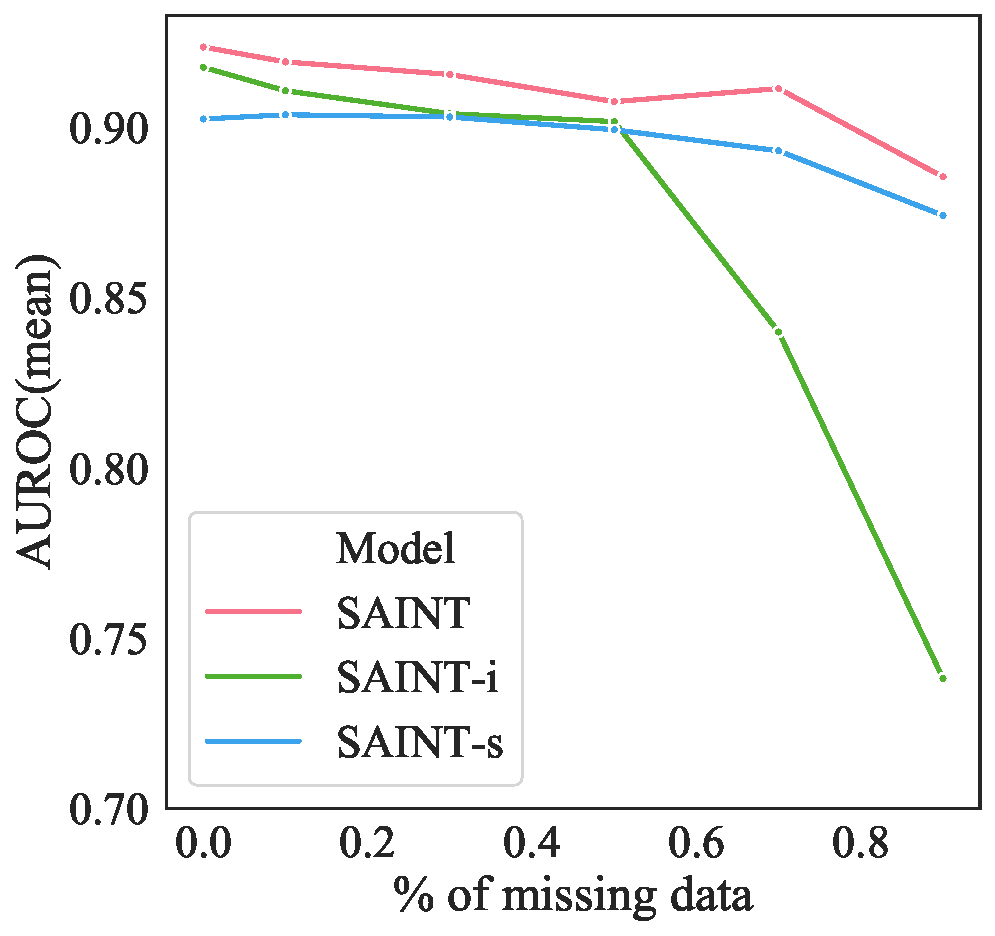
\includegraphics[width=\textwidth]{figs/appendix/missdata_plot.pdf}
         \caption{Trendlines of mean AUROC of SAINT's variants with varying \% of missing data.}
         \label{fig:missing_data_plot}
     \end{subfigure}
     \hfill
     \begin{subfigure}[b]{0.48\textwidth}
         \centering
         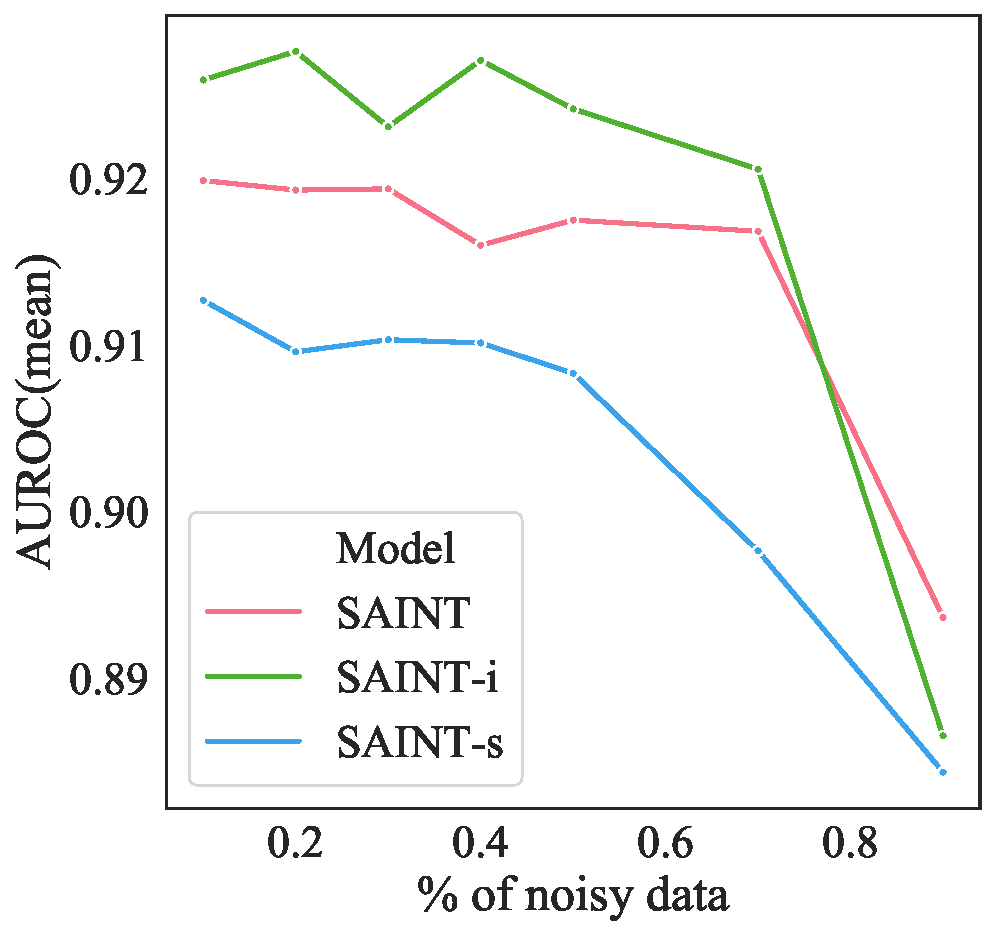
\includegraphics[width=\textwidth]{figs/appendix/noisydata_plot.pdf}
         \caption{Trendlines of mean AUROC of SAINT's variants with varying \% of noisy data.}
         \label{fig:noisy_data_plot}
     \end{subfigure}
     \caption{Robustness of SAINT's variants to data corruptions.}
     \label{fig:SAINT_robustness}
\end{figure}

\paragraph{Corrupted training data} We show in Figure~\ref{fig:SAINT_robustness} how the mean AUROC varies as we vary the percentage of the training data that is corrupted. We consider 2 types of corruptions - missing data as shown in Figure~\ref{fig:missing_data_plot} and noisy data as shown in Figure~\ref{fig:noisy_data_plot}. We observe that the SAINT model is quite robust across both variants, and the drop in performance is minimal until 70\% of training data is corrupted. We also observe that the self-attention variant SAINT-s is more robust in the case of missing data, while the intersample attention variant SAINT-i is more robust in case of noisy data. 

\paragraph{Effect of batch size on intersample attention performance (cont.)}

As discussed in the main body, we examine the affect of batch size on different SAINT variants in Figure ~\ref{fig:batchsize_ablation}. We pick 5 datasets with varying numbers of features and samples. In all cases, we see that the variance in AUROC is minimal when varying the batch size from 32 to 256.
\begin{figure}[h]
  \centering
  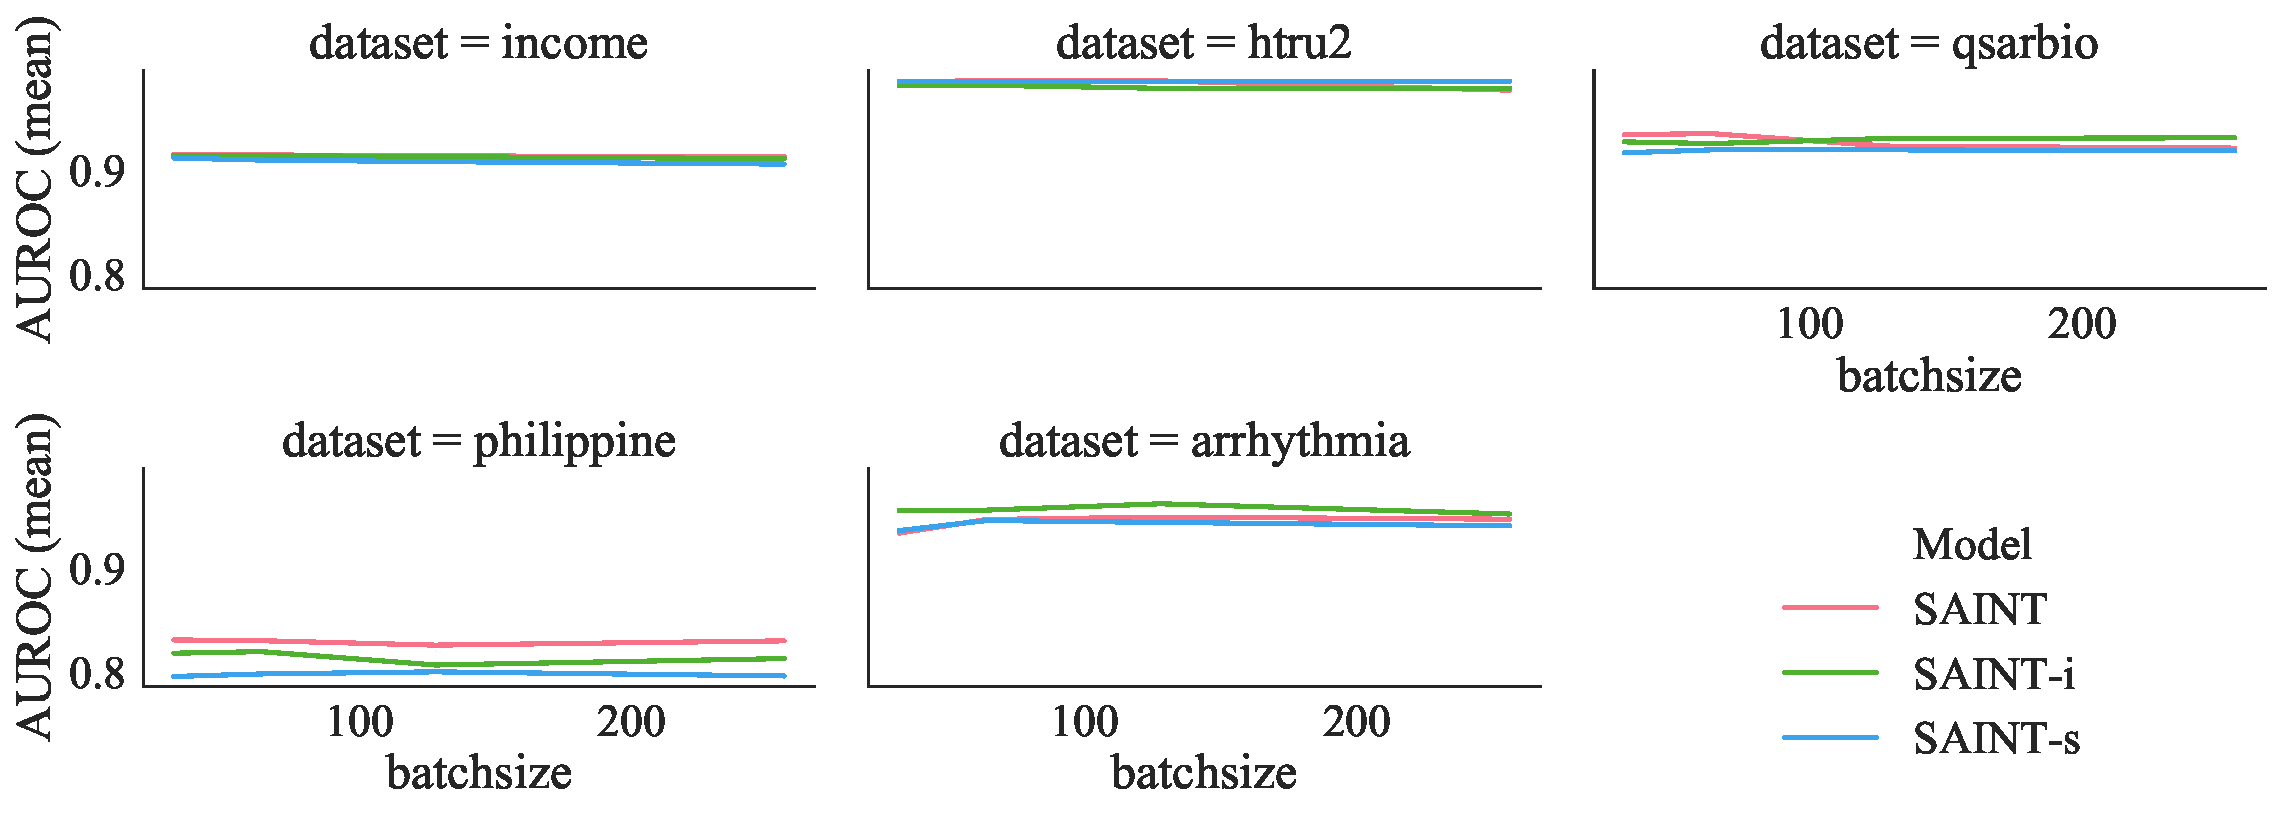
\includegraphics[width=\textwidth]{figs/appendix/batch_size_ablation.pdf}
  \caption{Trend lines of AUROC with varying training batch size. Results shown for 5 datasets}
  \label{fig:batchsize_ablation}
\end{figure}
\subsection{Pre-training Ablations}

In Table~\ref{table:pt_ablation}, we study various configurations of pre-training components. We perform 3 primary studies: we vary (1) projection head, (2) pre-training loss, and (3) data augmentation method. Note, the final result in all 3 studies refers to the same experiment (hence the row is repeated), which is the final chosen configuration for our model. In addition to the table, in Figure ~\ref{fig:temp_ablation}, we study the connection between the temperature $\tau$ and the type of projection head.
\begin{table}[h!]
\centering
\captionsetup{width=0.7\textwidth,font=small}
\captionof{table}{Ablation studies on the pre-training pipeline of SAINT. We break down the effect of the projection head, pre-training loss, and augmentation method. We report average AUC (in \%) over 14 datasets for the case where only 50 points in the dataset are labeled. }
\resizebox{0.7\textwidth}{!}{

\begin{tabular}{c|c|ccc}
\toprule
Study              & Variation                & SAINT-s     & SAINT-i     & SAINT\\
 \toprule
\multirow{3}{*}{1} & no proj. head            & 84.26 & 83.56 & 84.90   \\
                   & weight sharing head & 85.31 & 85.20 & 86.89   \\
                   & w. diff proj. head & \textbf{86.02} & \textbf{85.26} & \textbf{86.96}   \\
\midrule
\multirow{5}{*}{2} & no pre-training          & 85.14 & 83.93 & 85.78   \\
                   & contrastive             & 85.40 & 84.42 & 85.58   \\
                   & denoising               & 84.74 & 84.93 & 86.21   \\
                   & cosine similarity               & 85.03 & 84.35 & 85.70   \\
                   & contra. + denois.  & \textbf{86.02} & \textbf{85.26} & \textbf{86.96}   \\
\midrule
\multirow{3}{*}{3} & CutMix                  & 82.80 & 84.61 & 85.37  \\ 
                   & mixup                   & 86.01 & 84.41 & 86.45   \\
                   & CutMix + mixup          & \textbf{86.02} & \textbf{85.26} & \textbf{86.96}   \\
\bottomrule
\end{tabular}
}

\label{table:pt_ablation}
\end{table}

\textbf{Effect of projection heads:} As described in Section \ref{sec:pretraining}, we use two different projection heads, $g_1(\cdot)$ and $g_2(\cdot)$, to project the contextual representations to lower dimensions and then compute contrastive losses. We study three different options for the heads: (1) distinct projection heads (2) heads with weight sharing, and %\tom{Do you mean to say shared weights?  What does same mean?}\gowthami{Yes, they share weights}
(3) no projection heads at all. Table~\ref{table:pt_ablation} shows that using distinct projection heads performs best.

\textbf{Varying pre-training loss:} We train SAINT's variants with different loss functions, as shown in Study 2 of Table~\ref{table:pt_ablation}. We try denoising and contrastive losses, in addition to a cosine similarity loss on positive pairs (inspired by \cite{grill2020bootstrap, chen2020exploring}). The combination of contrastive and denoising consistently yields the best results in all SAINT variants.

\textbf{Varying the pre-training augmentations:} We also try to understand how important it is to use CutMix and mixup to generate augmented embeddings in the pre-training pipeline. We tinker with various configurations in Study 3 of Table~\ref{table:pt_ablation}, and we observe that using these two augmentations in unison results in the best performance across all SAINT variants.

\begin{figure}[h]
  \centering
  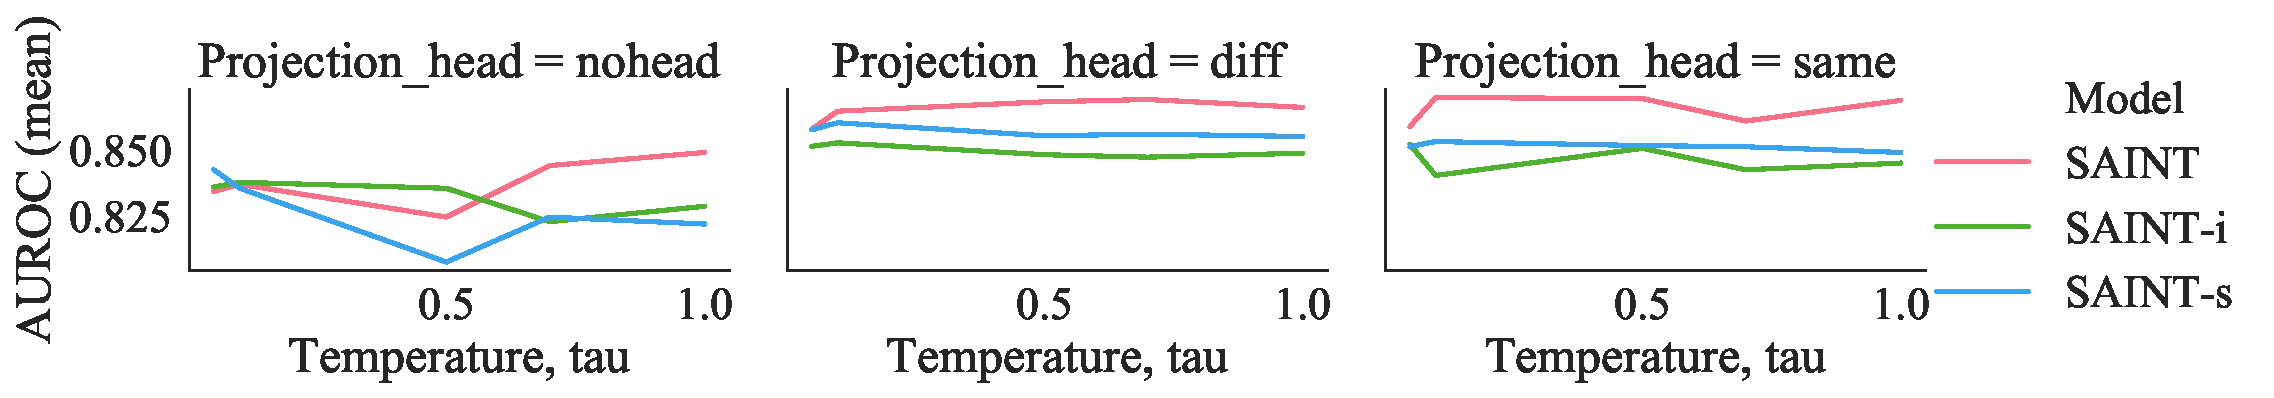
\includegraphics[width=\textwidth]{figs/appendix/temperature_ablation.pdf}
  \caption{Temperature and Projection head ablation}
  \label{fig:temp_ablation}
\end{figure}



% \paragraph{Varying temperature plots}

\section{Additional interpretability plots}
\label{appendix_sec:additional_interpret}

In Figure~\ref{fig:SA_in_SAINTs_mnist}, we show a self-attention plot for the SAINT-s variant (with $L=1$) on MNIST. The self-attention in one stage SAINT-s model behaves similar to a one stage SAINT model. However, when there are more stages, the attention in the last stage is not quite as interpretible.

In Figure~\ref{fig:ISA_in_SAINT_volkert}, we show the intersample attention between a batch of points from different classes in SAINT model on the Volkert dataset. Similarly in Figure~\ref{fig:ISA_in_SAINTi_volkert}, we show intersample attention in the SAINT-i variant on the same batch of points from the Volkert dataset. As mentioned in the main body, the intersample behaviour is not quite as sparse as that of MNIST. We hypothesize that the sparsity of the intersample attention layer depends on how separable the classes in the dataset are. (Volkert is a harder dataset than MNIST).


In Figure~\ref{fig:attention_tsne_volkert}, we show the t-SNE plots on value vectors for SAINT and SAINT-i variants on Volkert. Unlike MNIST, all the classes are attended to equally.

\begin{figure}[h]
     \centering
     \begin{subfigure}[b]{0.3\textwidth}
         \centering
         ~\vspace{4mm}
         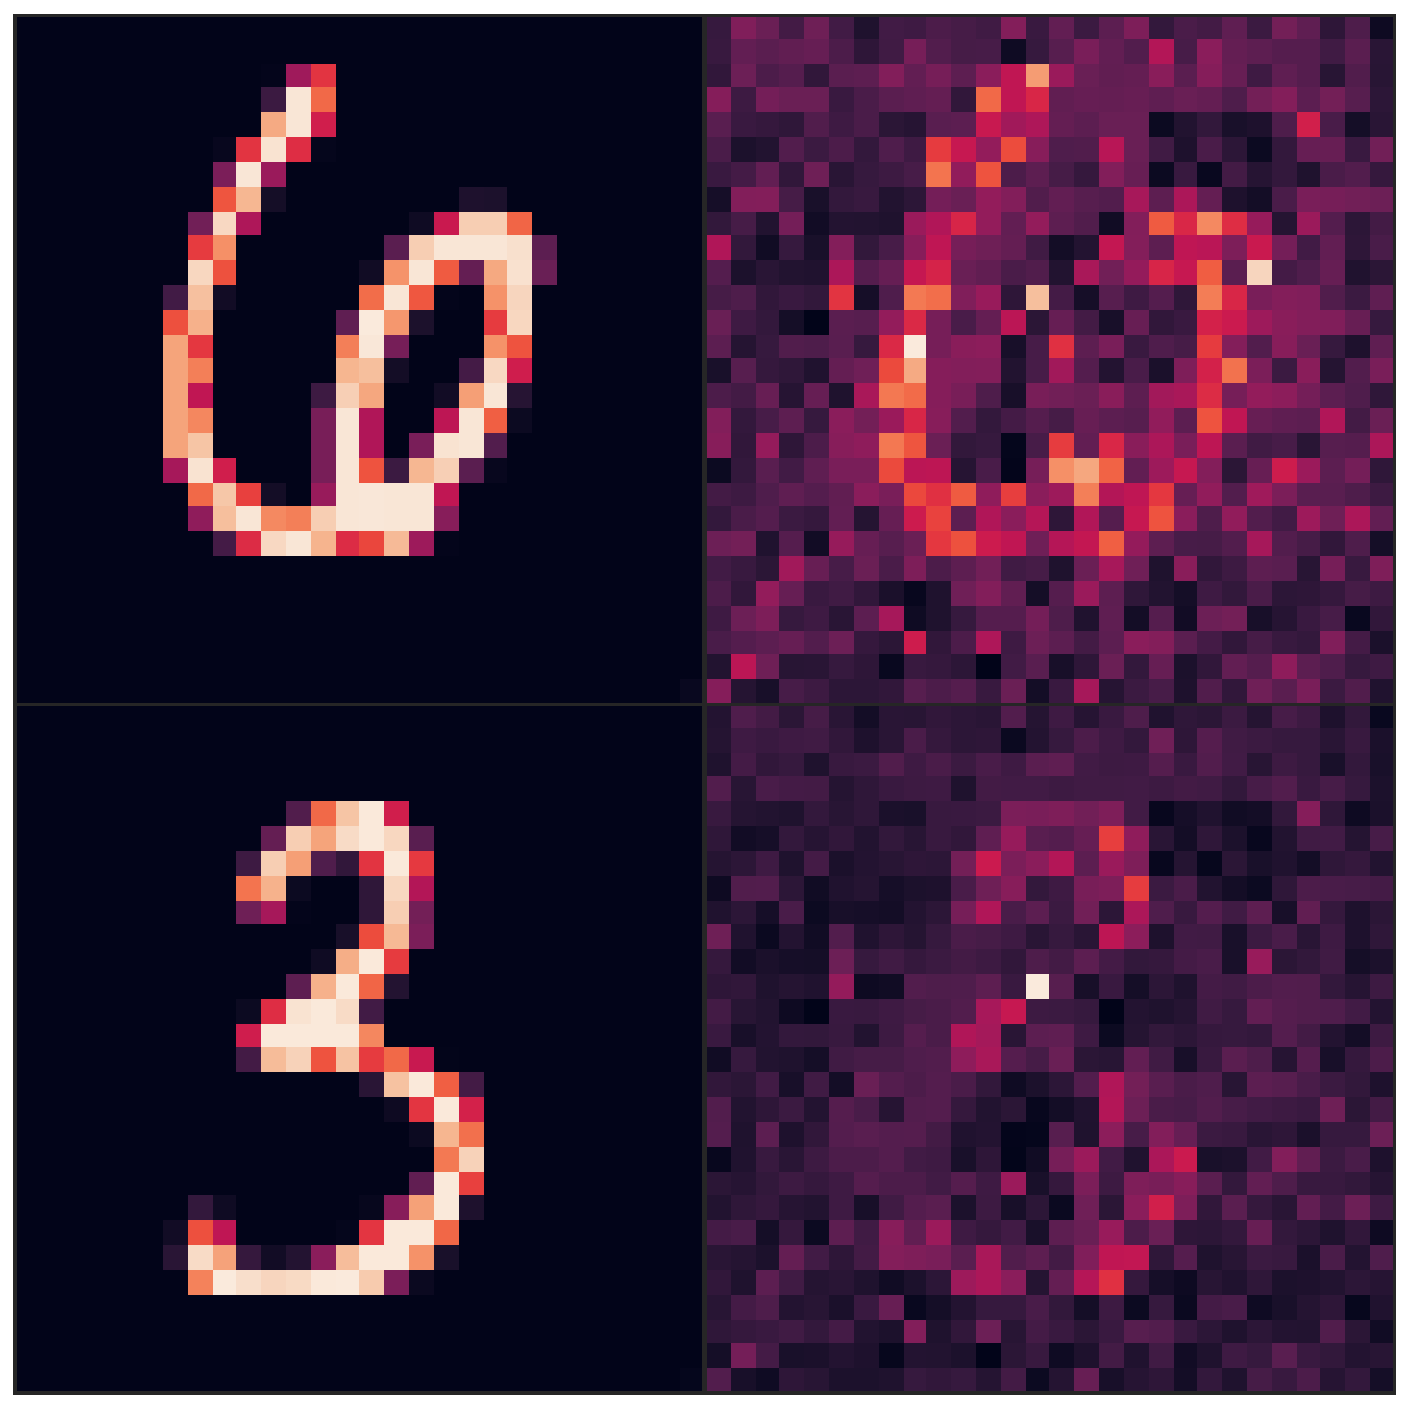
\includegraphics[width=\textwidth,valign=t]{figs/appendix/col_col_attention.pdf}
         \caption{Self-attn. in 1 layered SAINT-s on MNIST dataset}
         \label{fig:SA_in_SAINTs_mnist}
     \end{subfigure}
     \hfill
     \begin{subfigure}[b]{0.32\textwidth}
         \centering
         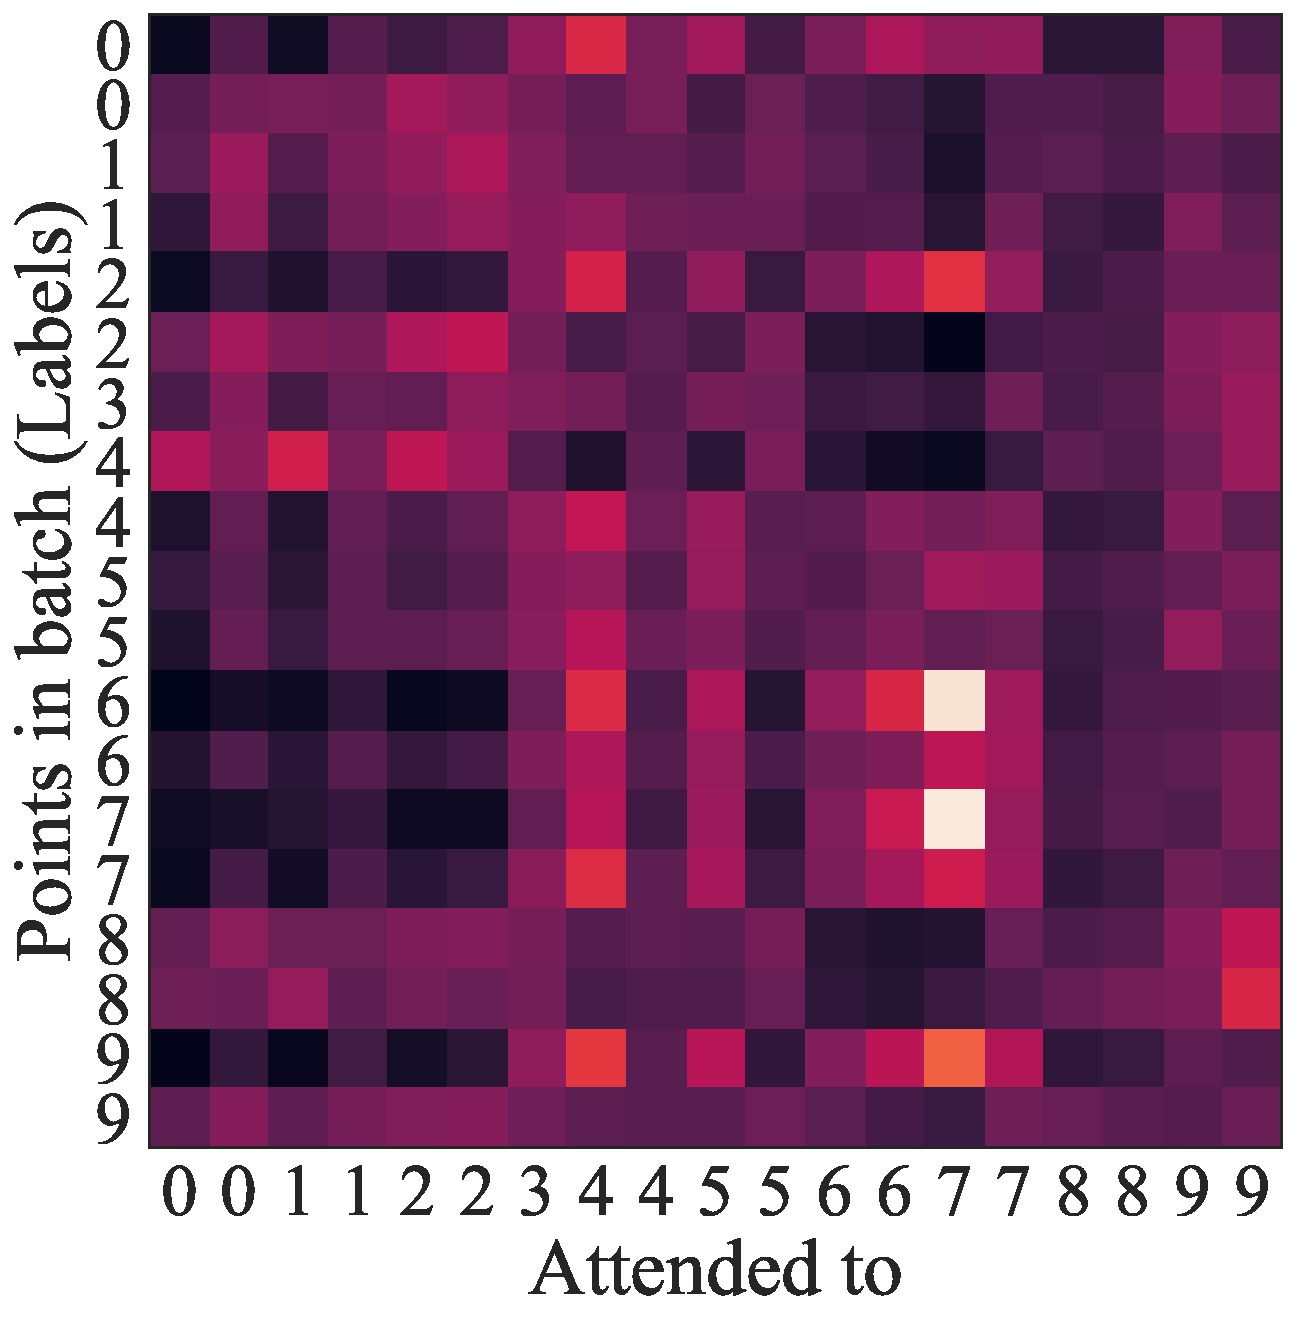
\includegraphics[width=\textwidth,valign=t]{figs/appendix/volkert/volkert_Row_colrow_onebatch.pdf}
         \caption{Intersample attn. in SAINT in Volkert dataset}
         \label{fig:ISA_in_SAINT_volkert}
     \end{subfigure}
     \hfill
     \begin{subfigure}[b]{0.32\textwidth}
         \centering
         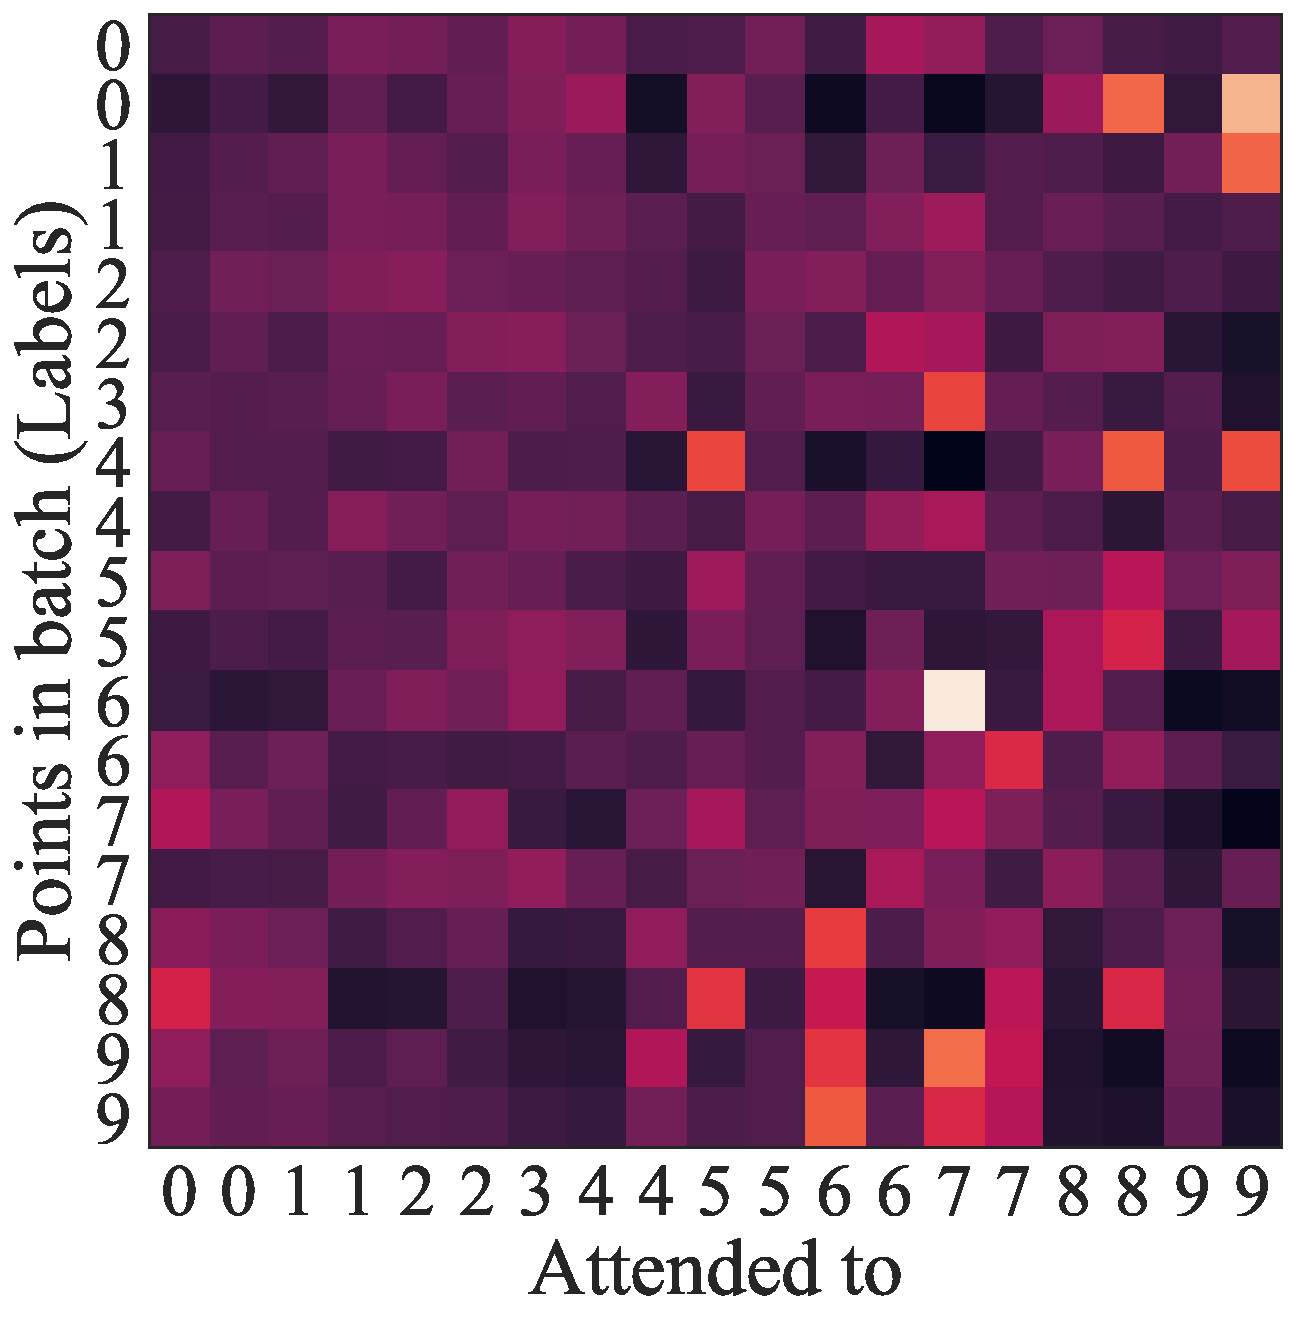
\includegraphics[width=\textwidth,valign=t]{figs/appendix/volkert/volkert_Row_row_onebatch.pdf}
         \caption{Intersample attn. in SAINT-i in Volkert dataset} 
         \label{fig:ISA_in_SAINTi_volkert}
     \end{subfigure}
     \captionsetup{font=small}
        \caption{Visual representations of various attention mechanisms. (a) Self-attention in SAINT-s on MNIST (b,c) Intersample attention in SAINT and SAINT-i on the Volkert dataset. }
        \label{fig:appendix_attention_plots}
\end{figure}

\begin{figure}[h]
    \centering
     \begin{subfigure}[b]{0.45\textwidth}
         \centering
         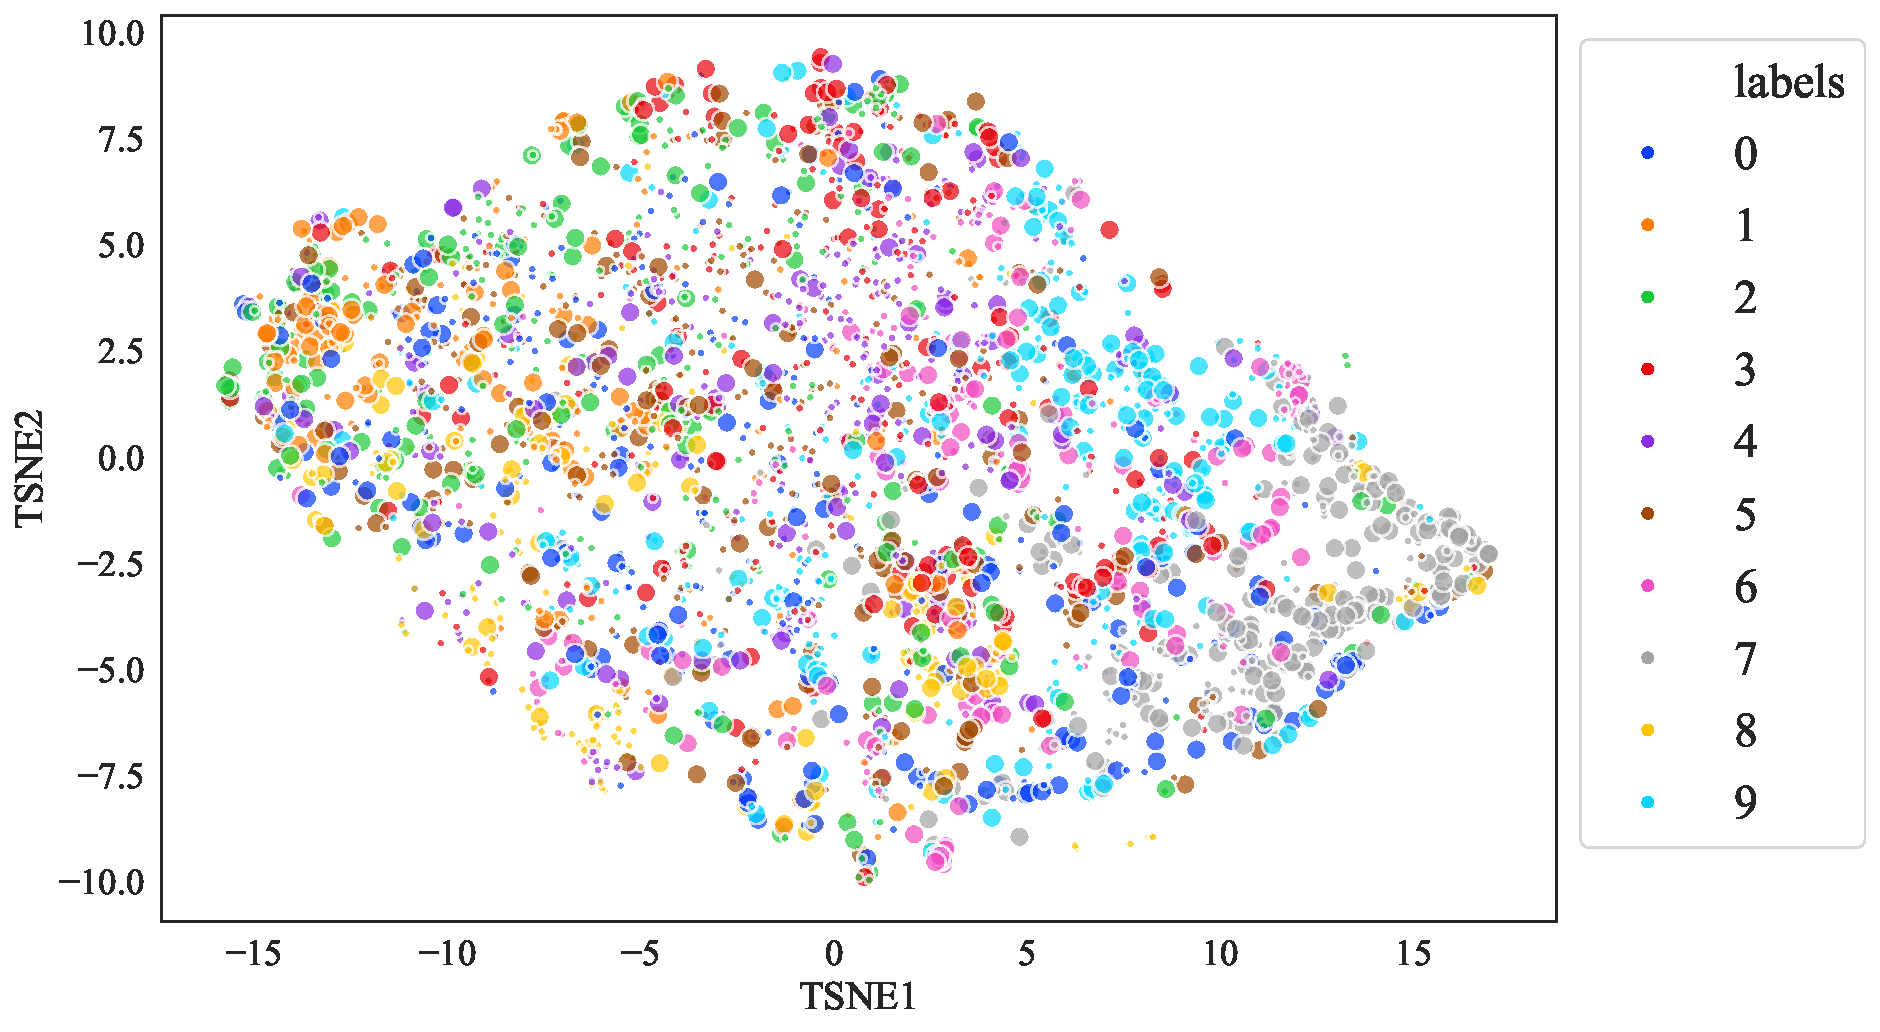
\includegraphics[width=\textwidth]{figs/appendix/volkert/volkert_Row_colrow_tsne.pdf}
         \label{fig:saint_tsne_volkert}
     \end{subfigure}
     \begin{subfigure}[b]{0.45\textwidth}
         \centering
         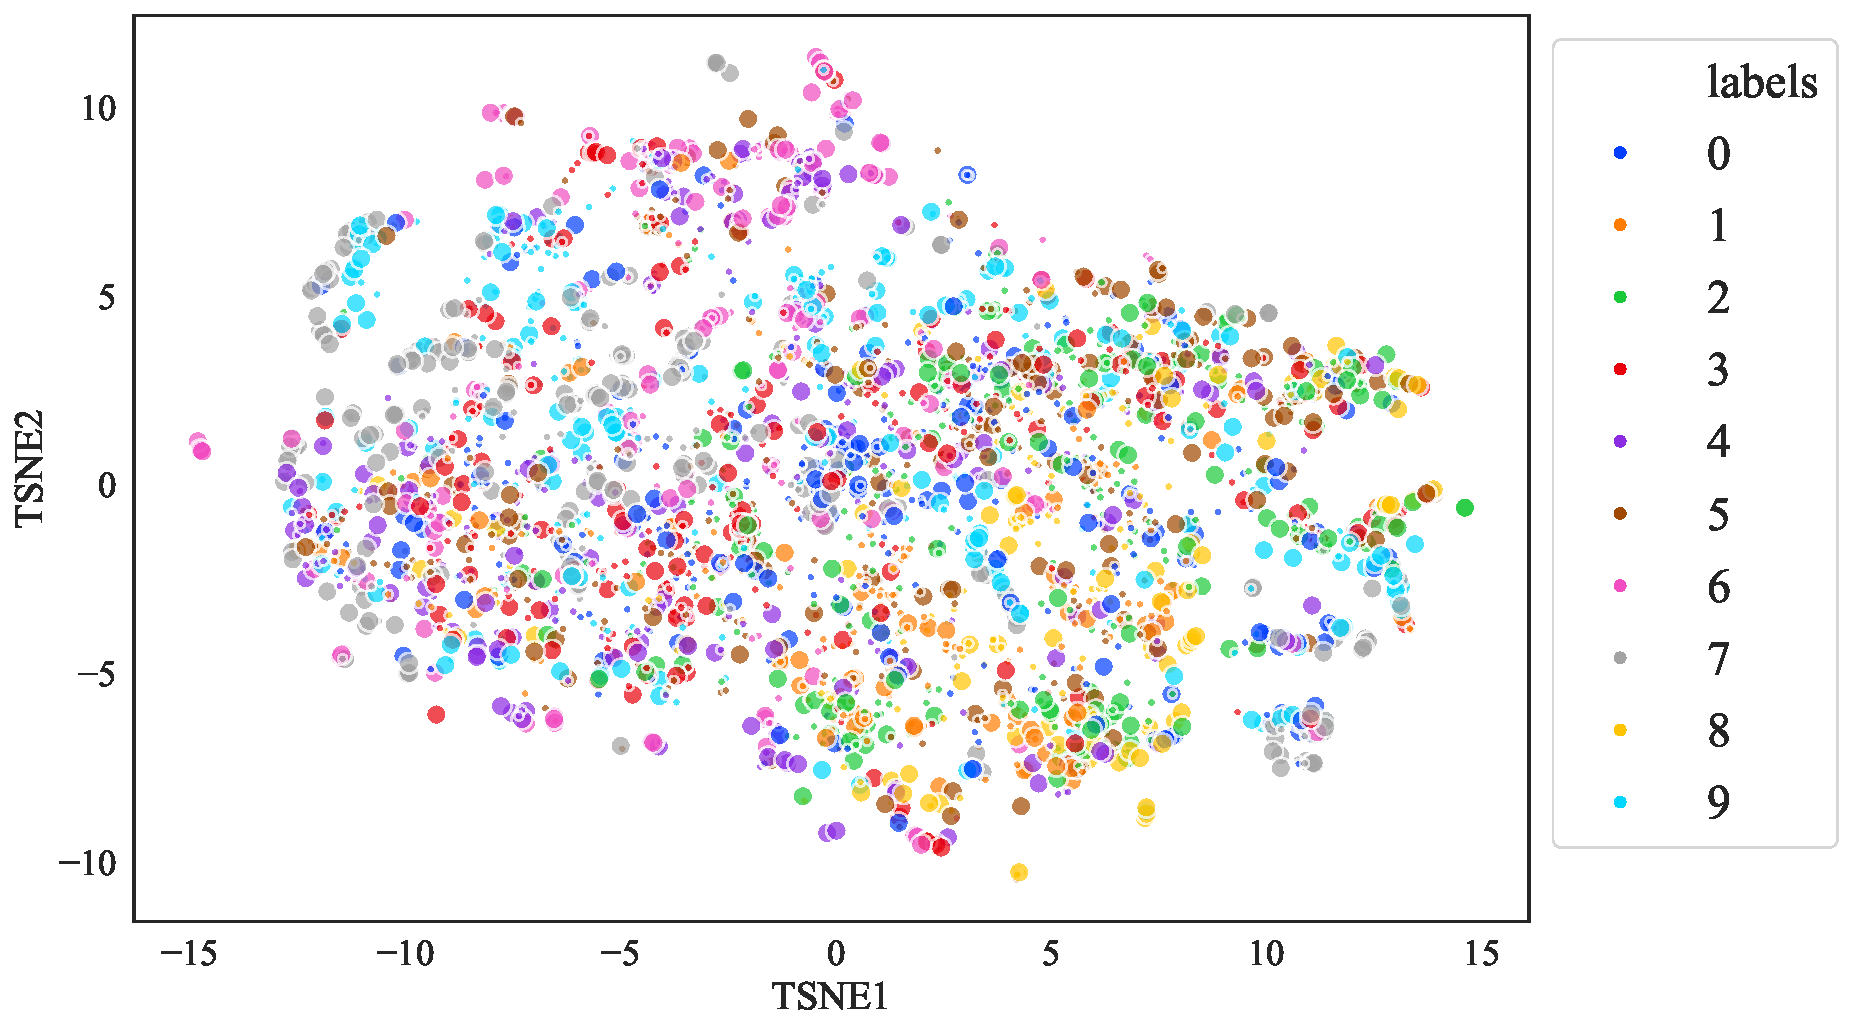
\includegraphics[width=\textwidth]{figs/appendix/volkert/volkert_Row_row_tsne.pdf}
         \label{fig:saint_i_tsne_volkert}
     \end{subfigure}
     \captionsetup{font=small}
     \vspace{-5mm}
    \caption{A t-SNE visualization of \textit{value} vectors in intersample attention layers of SAINT~(left) and SAINT-i~(right) on the Volkert dataset. We plot 3000 points in each figure, with classes uniformly represented. Unlike MNIST, all classes are uniformly attended to in this dataset.}
    \label{fig:attention_tsne_volkert}
\end{figure}


% {
% \small
% \bibliographystyle{plainnat}
% \bibliography{references}
% }

% \end{document}